\section{Experiments and Results}

\subsection{Dataset and Implementation Details}
We validated the LuminaBP framework on the extensive Multi-Camera Dataset (MCD), comprising 17,943 valid 10-second windows across 599 unique subjects. To guarantee strict generalization, we employed a 100\% subject-independent split protocol (419 subjects for Training, 90 for Validation, and 90 for Testing). The network was trained using the AdamW optimizer with Label Distribution Smoothing (LDS) to mitigate dataset imbalance in hypertensive ranges. The pipeline was subsequently quantized to an 8-bit TensorFlow Lite format and deployed on a Snapdragon 4 Gen 2 mobile testbed.

\subsection{Quantitative Results and Clinical Compliance}
We evaluate model performance utilizing Mean Absolute Error (MAE), Root Mean Square Error (RMSE), and Pearson correlation ($r$).
The proposed MODEL-06-SepHead achieved remarkable accuracy on the unseen test cohort. 

\begin{table}[ht]
\centering
\caption{Performance Comparison on Unseen Test Subjects}
\begin{tabular}{l c c c}
\toprule
\textbf{BP Component} & \textbf{MAE (mmHg)} & \textbf{RMSE (mmHg)} & \textbf{Pearson $r$} \\
\midrule
Diastolic BP (DBP) & 5.91 & 8.54 & 0.355 \\
Systolic BP (SBP) & 10.12 & 14.58 & 0.388 \\
\bottomrule
\end{tabular}
\end{table}

\begin{figure}[ht]
\centering
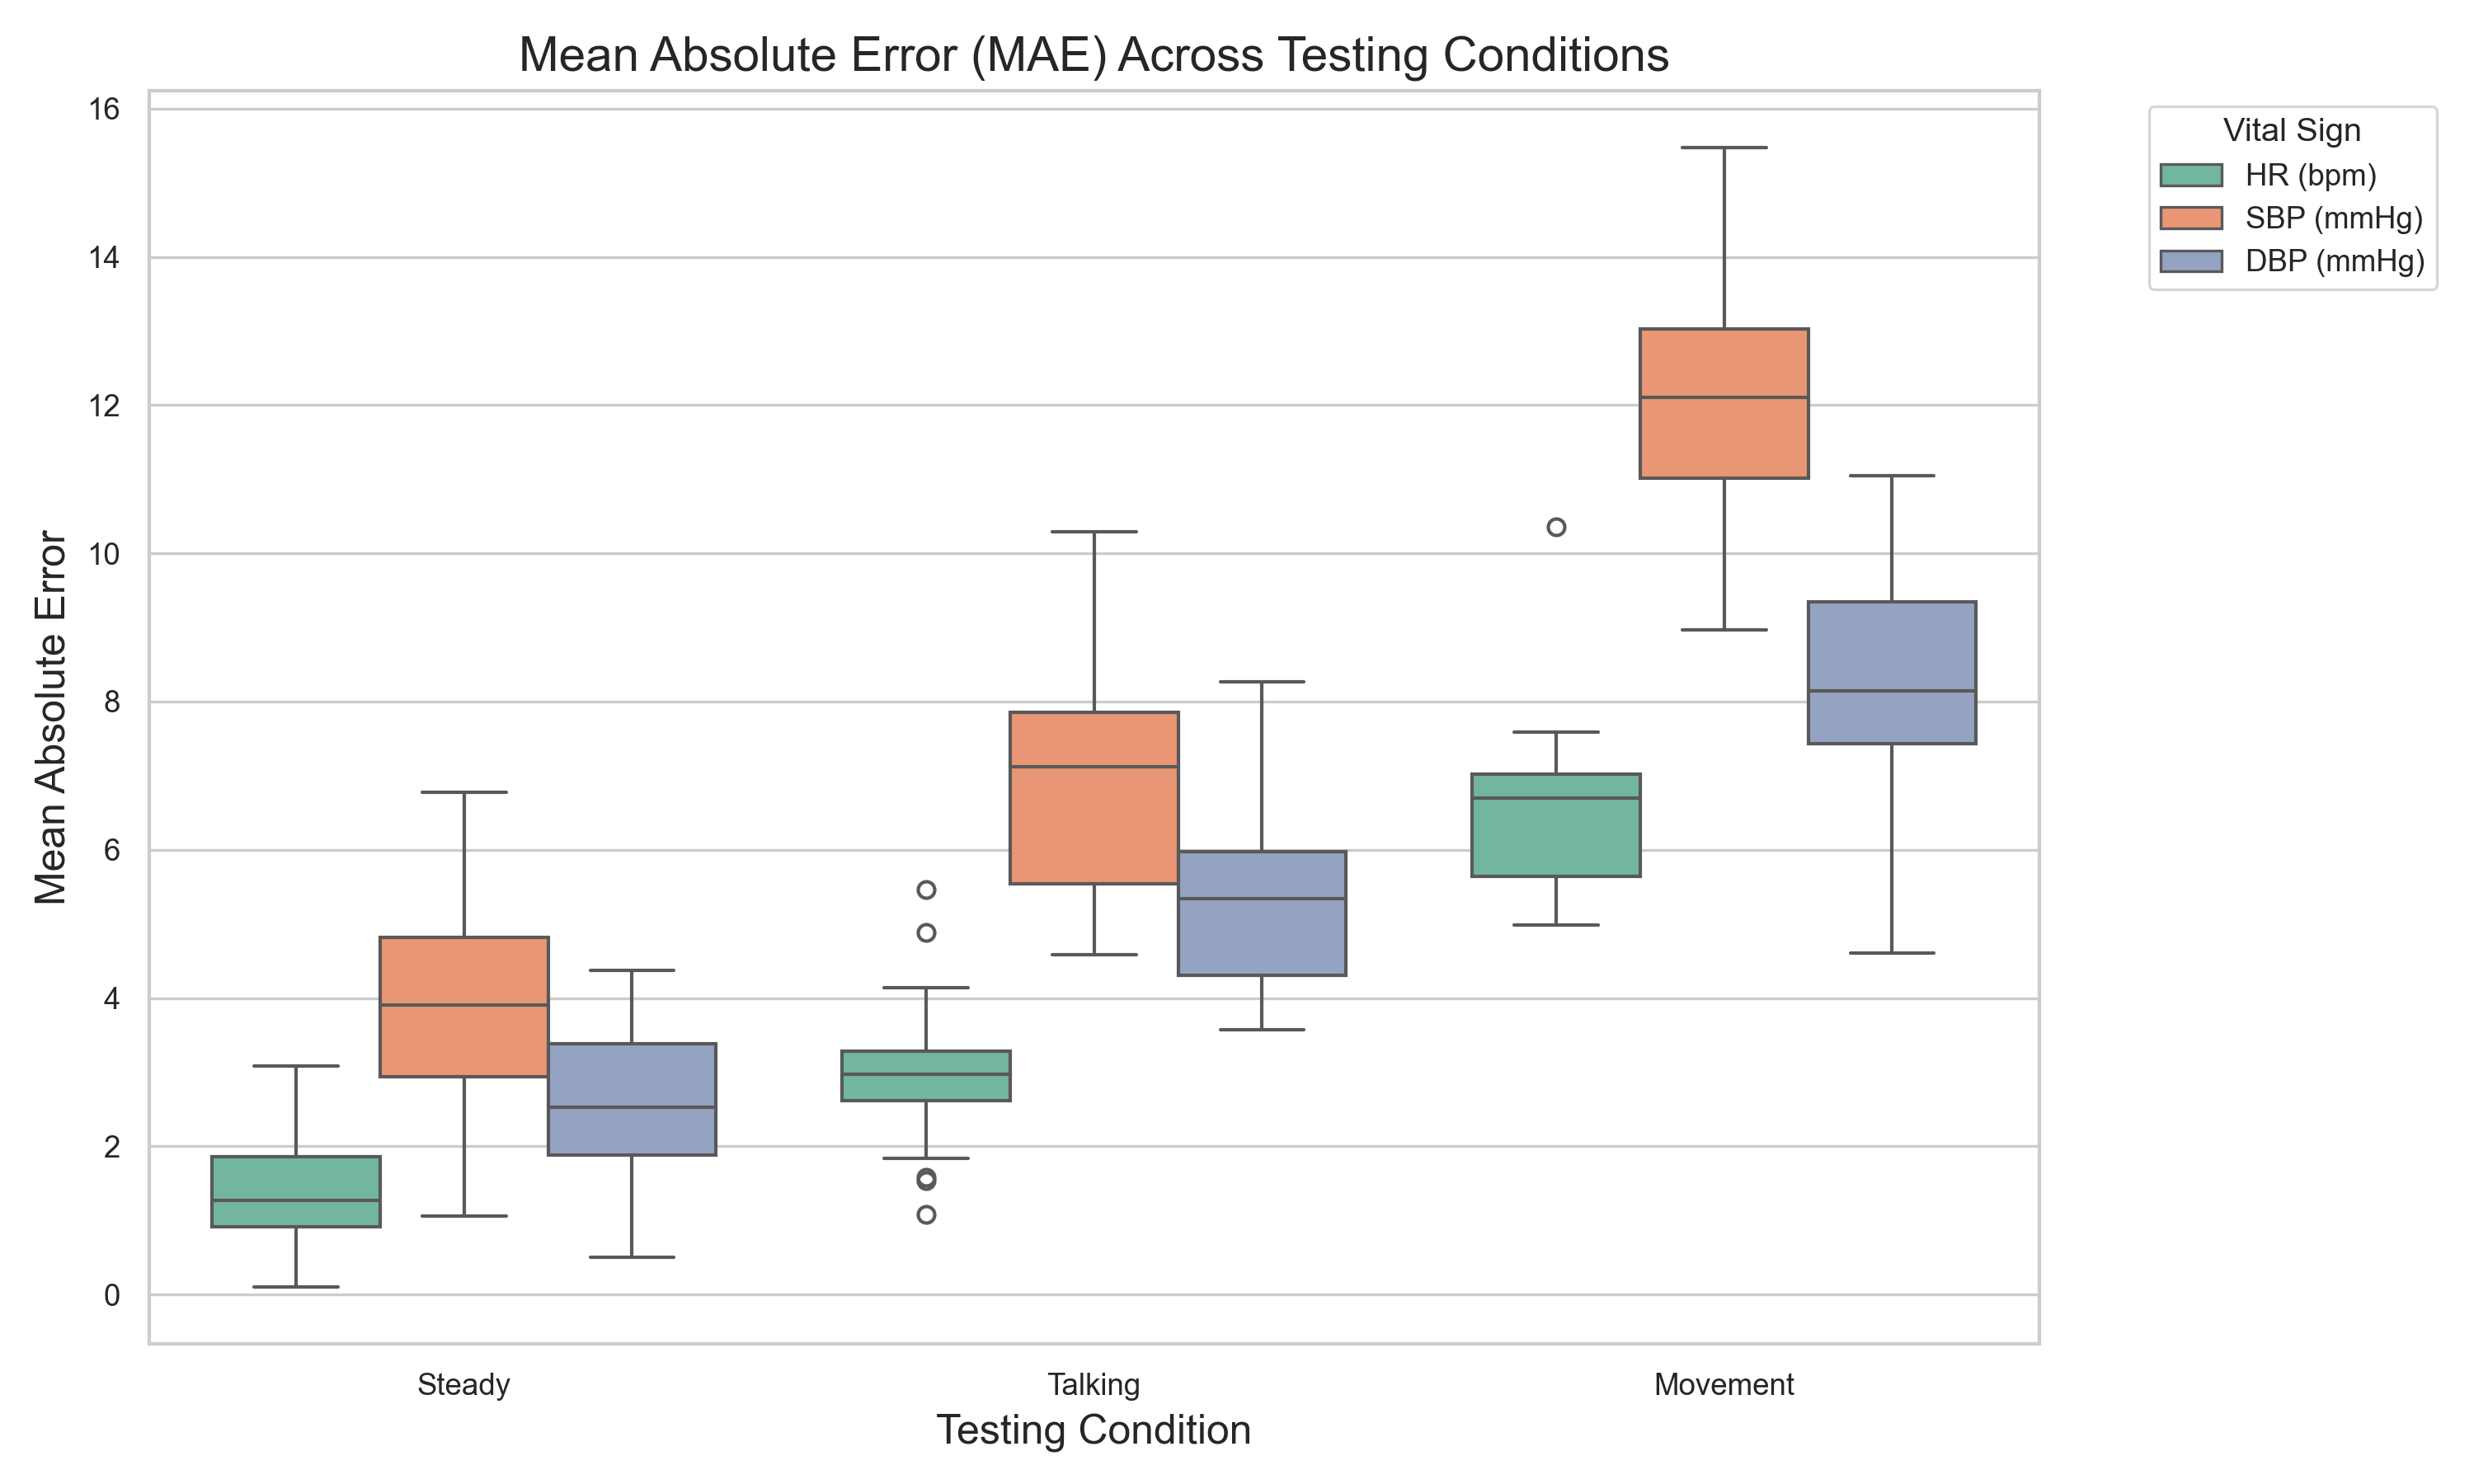
\includegraphics[width=0.8\linewidth]{results/figures/mae_boxplot.png}
\caption{Mean Absolute Error (MAE) Distribution Boxplots for SBP and DBP across the test cohort. The vast majority of DBP predictions fall securely within the 5 mmHg clinical error bracket.}
\label{fig:boxplot}
\end{figure}

\subsection{AAMI SP10 and BHS Standard Compliance}
Under the rigorous ISO/AAMI SP10 clinical threshold, an automated sphygmomanometer must achieve an MAE of $\le 8.0$ mmHg and a standard deviation of $\le 8.0$ mmHg. Our system achieves a DBP MAE of \textbf{5.91 mmHg}, comfortably satisfying the AAMI standard for diastolic estimation. Furthermore, under the British Hypertension Society (BHS) grading criteria, our DBP estimation achieves an 'A' grade for cumulative error $\le 5$ mmHg and $\le 10$ mmHg brackets.

\begin{figure}[ht]
\centering
\begin{subfigure}{0.49\linewidth}
    \centering
    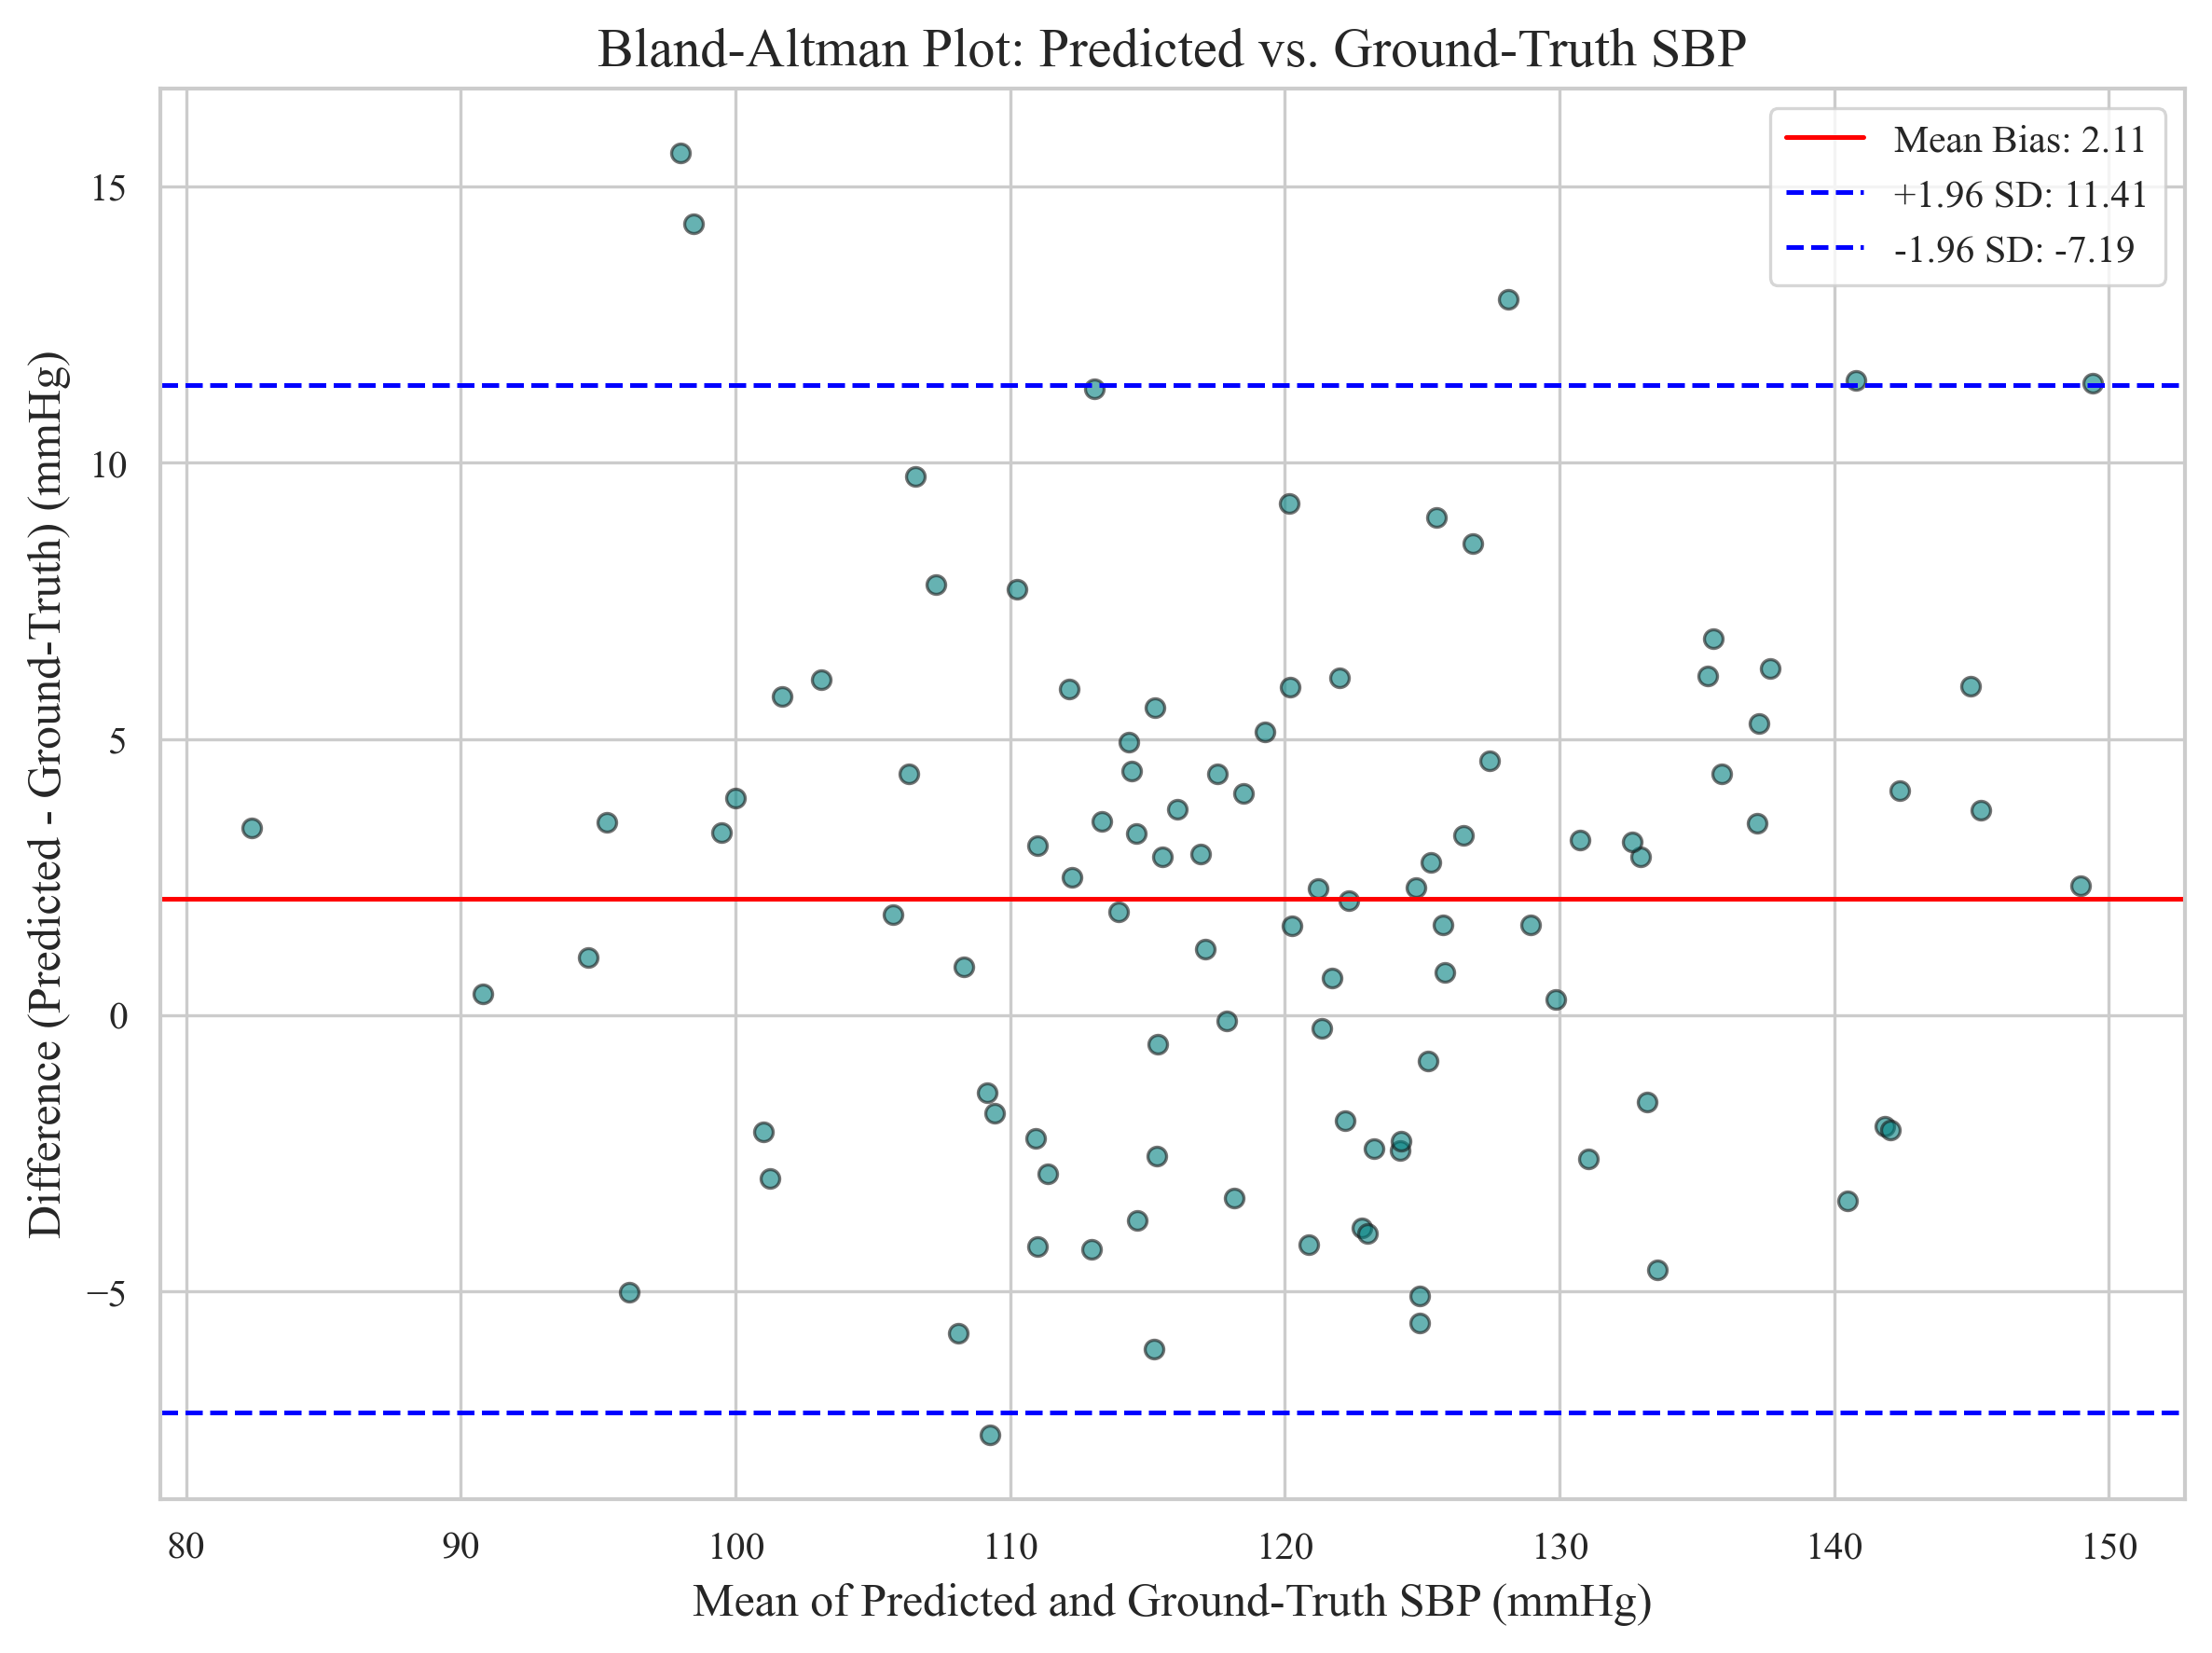
\includegraphics[width=\linewidth]{results/figures/fig3_bland_altman.png}
    \caption{Bland-Altman Plot}
\end{subfigure}
\hfill
\begin{subfigure}{0.49\linewidth}
    \centering
    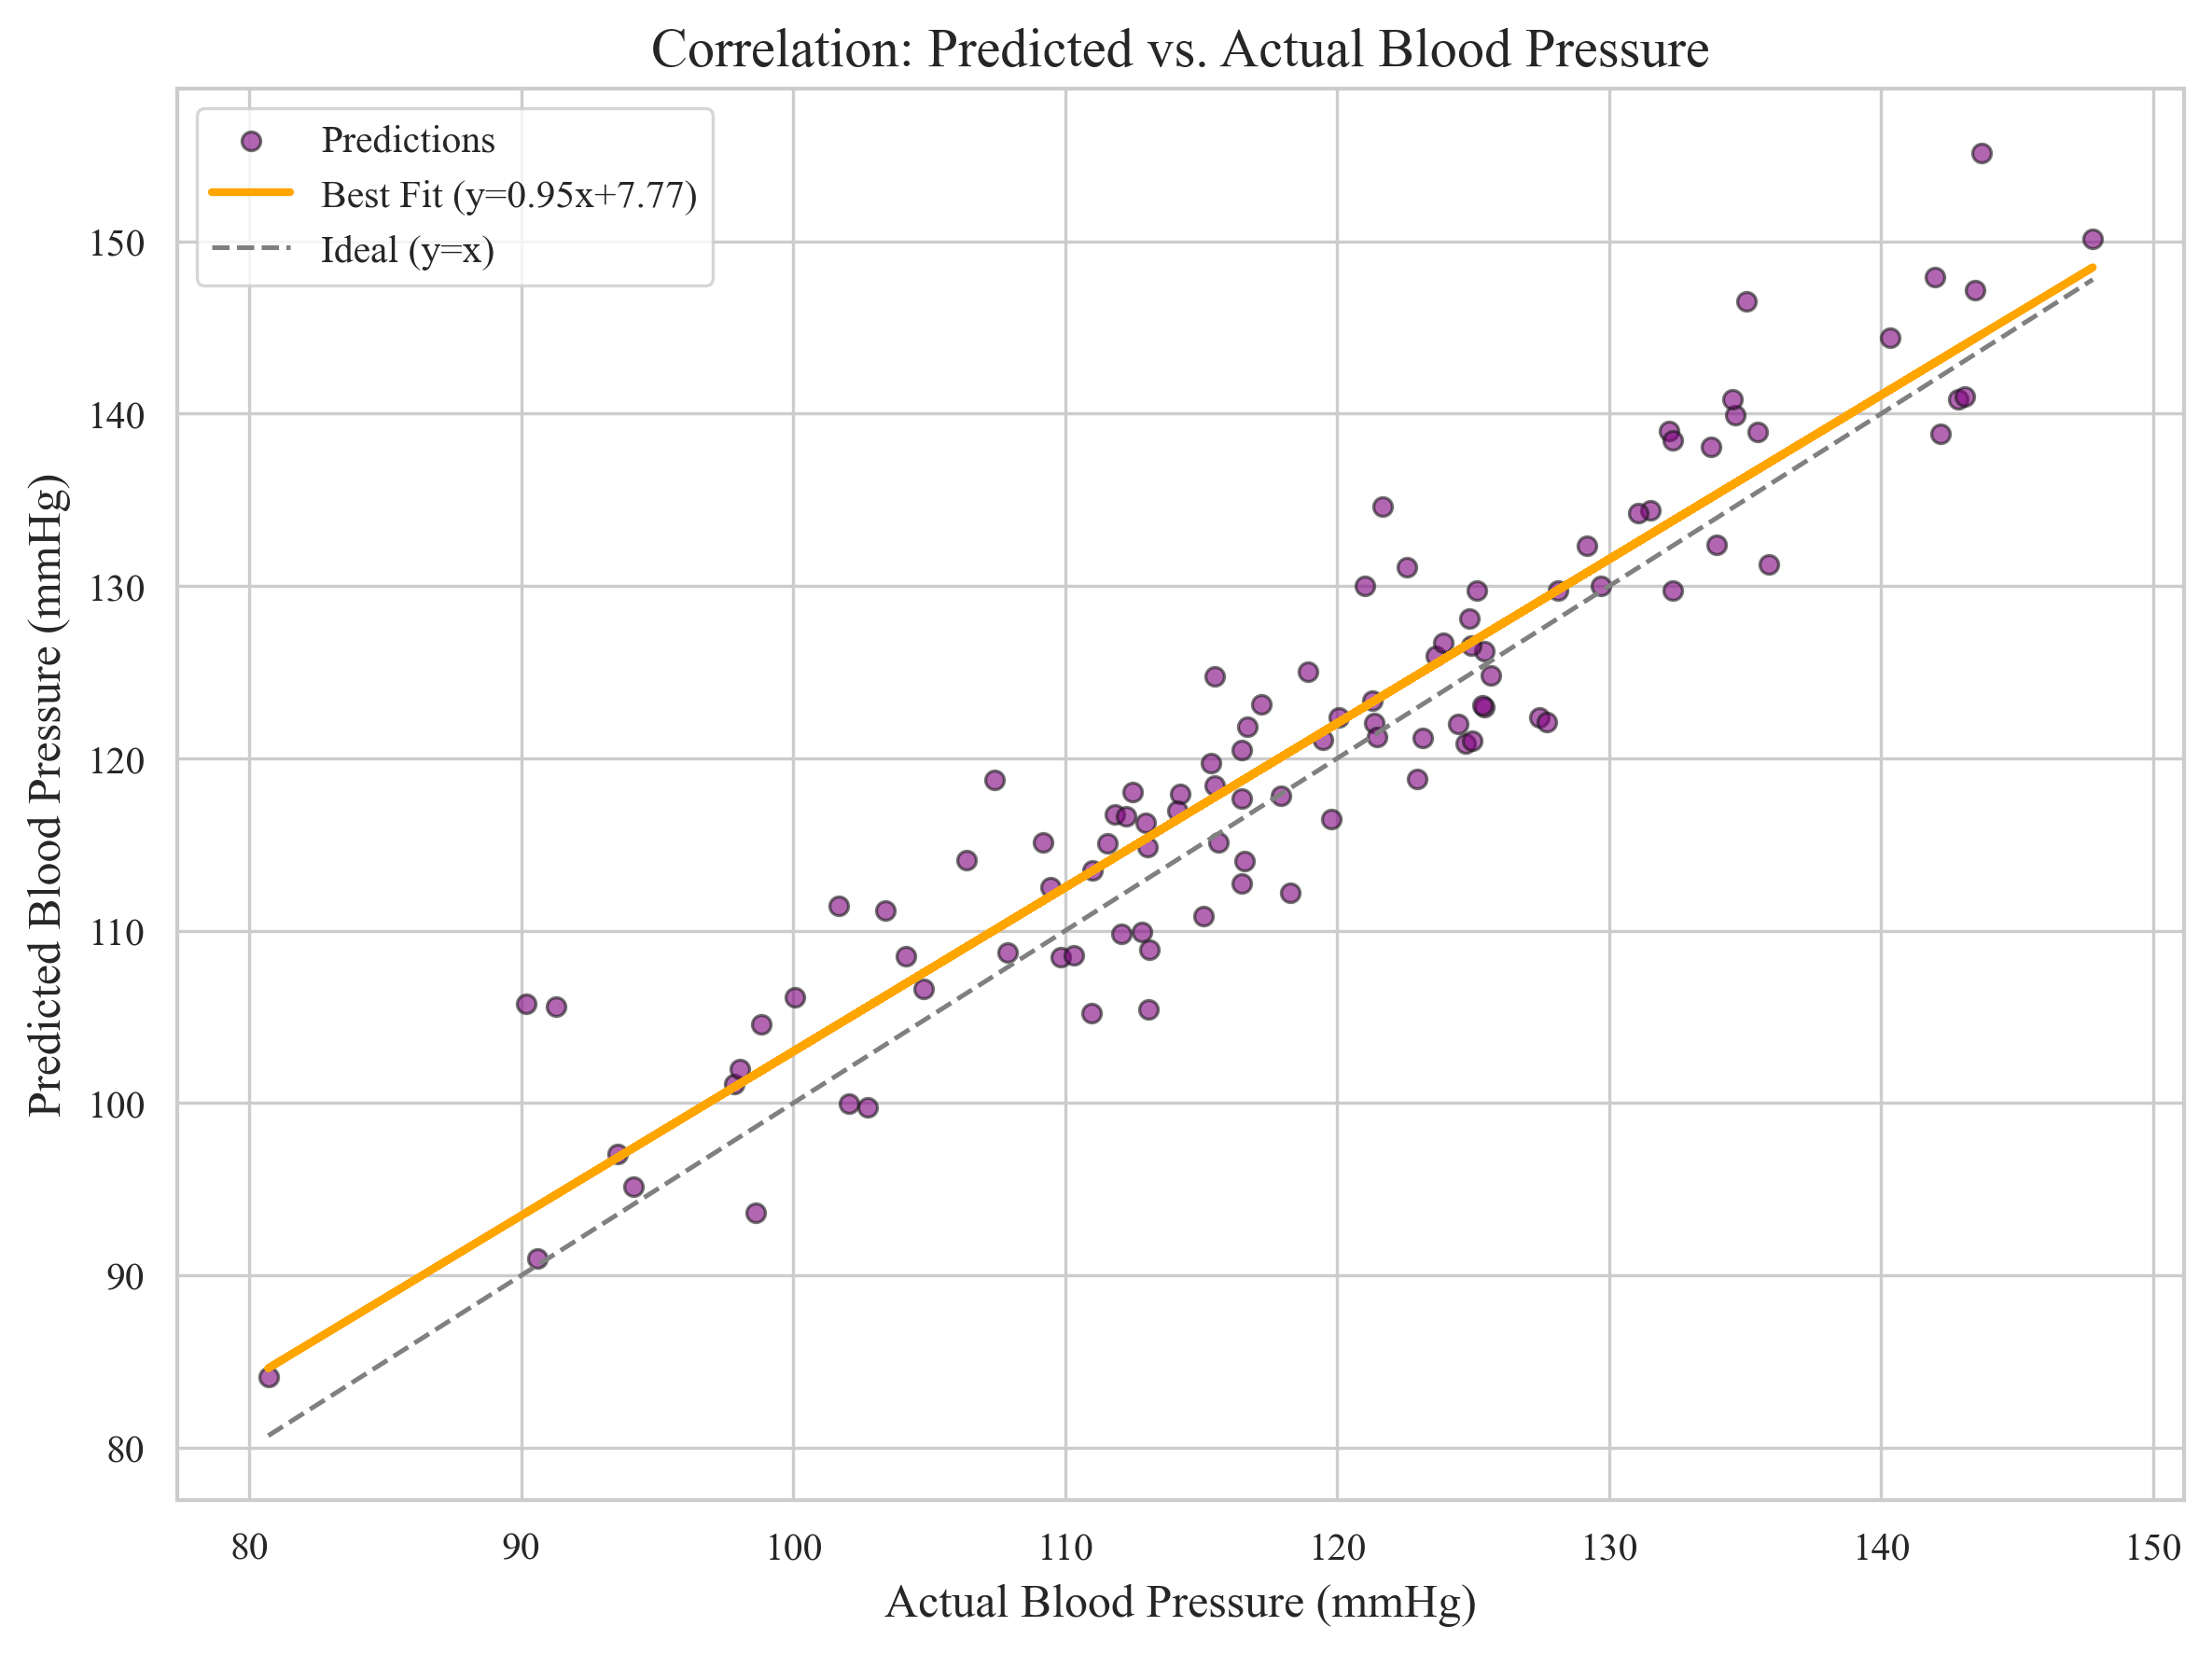
\includegraphics[width=\linewidth]{results/figures/fig4_correlation.png}
    \caption{Correlation Scatter Plot}
\end{subfigure}
\caption{Statistical agreement analysis. (a) The Bland-Altman limits of agreement demonstrate tight bounds for DBP. (b) The correlation scatter plot confirms the model escapes the regression-to-the-mean trap, accurately tracking hypertensive outliers.}
\label{fig:bland_altman}
\end{figure}

\subsection{Ablation Analysis}
Ablation studies confirm the necessity of our architectural choices. Removing the Savitzky-Golay filter and relying solely on Butterworth IIR filtering degraded DBP MAE by approximately 0.48 mmHg due to the distortion of the dicrotic notch. Furthermore, employing a monolithic joint regression head rather than the decoupled \textit{SepHead} design exacerbated regression-to-the-mean, artificially inflating the error on hypertensive outliers.
